\begin{figure}[!htbp]
\begin{center}

\begin{subfigure}[b]{\linewidth}
\begin{center}

\begin{minipage}[t]{0.28\linewidth}
\centering
\vspace{0pt} % for alignment
\adjincludegraphics[width=\linewidth, trim={{.25\width} {.25\width} {.5\width} {.5\width}}, clip]{knockout/interior_propagule/wildtype/seed=1+title=directional_regulator_viz+treat=resource-wave__channelsense-yes__nlev-two+update=8188+_data_hathash_hash=8b493febd79aad1f+_script_fullcat_hash=90718bb0c6ec4dbd+_source_hash=53a2252-clean+ext=}
\footnotesize Wild type
\end{minipage}
\begin{minipage}[t]{0.28\linewidth}
\centering
\vspace{0pt} % for alignment
\adjincludegraphics[width=\linewidth, trim={{.5\width} {.5\width} {.25\width} {.25\width}}, clip]{knockout/interior_propagule/propaguleknockout/seed=1+title=directional_regulator_viz+treat=resource-wave__channelsense-yes__nlev-two+update=8188+_data_hathash_hash=2b6711db47fb5887+_script_fullcat_hash=90718bb0c6ec4dbd+_source_hash=53a2252-clean+ext=}
\footnotesize Propagule knockout
\end{minipage}
\begin{minipage}[t]{0.28\linewidth}
\centering
\vspace{0pt} % for alignment
\adjincludegraphics[width=\linewidth, trim={{.5\width} {.5\width} {.25\width} {.25\width}}, clip]{knockout/interior_propagule/regulationknockout/seed=1+title=directional_regulator_viz+treat=resource-wave__channelsense-yes__nlev-two+update=8188+_data_hathash_hash=11ab5cdd47ed18c7+_script_fullcat_hash=90718bb0c6ec4dbd+_source_hash=53a2252-clean+ext=}
\footnotesize Regulation knockout
\end{minipage}

\caption{Regulation visualizations}
\label{fig:regulation_visualizations}

\end{center}
\end{subfigure}

\begin{minipage}[t]{\linewidth}
\centering
\vspace{0pt} % for alignment
\begin{subfigure}[b]{\linewidth}
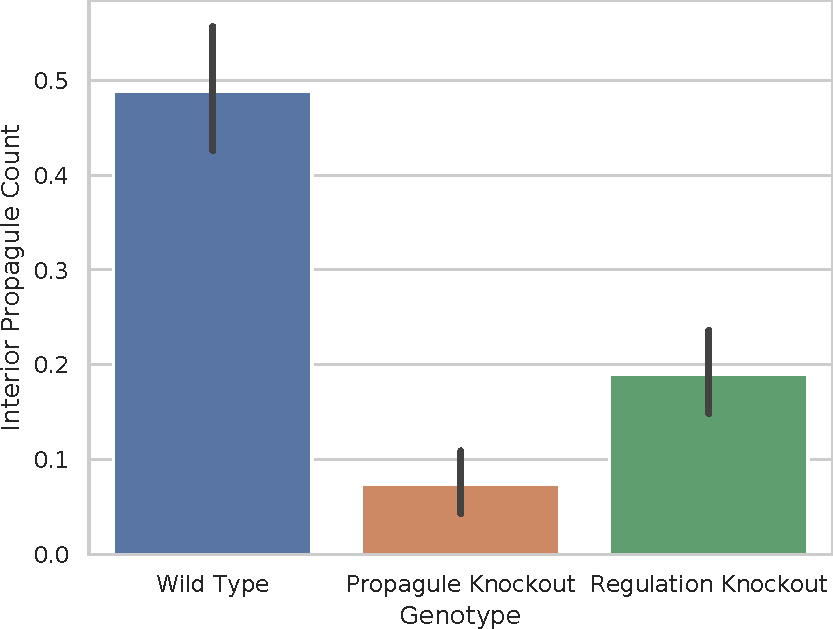
\includegraphics[width=\linewidth]{knockout/interior_propagule/title=interior_propagules+_data_hathash_hash=bb0fa6254f1b7398+_script_fullcat_hash=f738b363bea8c98a+_source_hash=53a2252-clean+ext=}%
\caption{Interior propagule rate by genotype}
\label{fig:interior_propagule_rate}
\end{subfigure}
\end{minipage}%
\hspace*{\fill}


\caption{
Comparison of a wild type strain evolved under the ``Nested-Wave'' treatment exhibiting interior propagule generation with knockouts of gene regulation and explicitly propagule-generating reproduction instructions.
Subfigures \ref{fig:interior_propagule-wt}, \ref{fig:interior_propagule-ko-regulation}, and \ref{fig:interior_propagule-ko-propagule} depict gene regulation at each of a cell's four directional SignalGP instances using a PCA mapping from regulatory state to three-dimensional RGB coordinates, calculated uniquely for each level-one same-channel signaling group.
Black borders divide level-one same-channel signaling groups and white borders divide level-zero same-channel signaling groups.
Figure \ref{fig:interior_propagule_rate} compares the mean number of interior propagules observed per level-one same-channel signaling group.
Error bars indicate 95\% confidence.
View an animation of wild type gene regulation at \url{https://mmore500.com/hopto/t}.
View the wild type strain in a live in-browser simulation at \url{https://mmore500.com/hopto/g}.
}
\label{fig:ko-interior_propagule}
\end{center}
\end{figure}
